\documentclass[tikz,border=2pt]{standalone}
\usepackage{pgfplots}
\usetikzlibrary{intersections}
\usepgfplotslibrary{fillbetween}
\pgfplotsset{compat=1.7}

\begin{document}
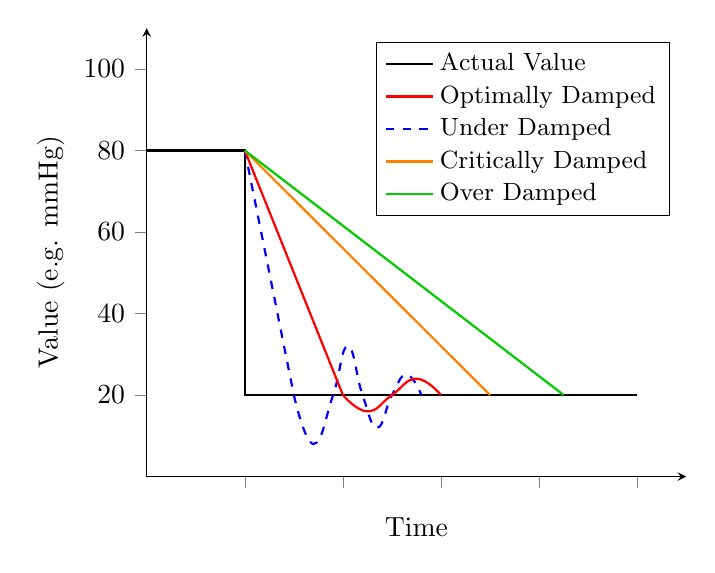
\begin{tikzpicture}


\begin{axis}[
        axis lines=middle,
        grid style={none},
	ymin = 0,
	ymax = 110,
	xmin = 0,
	xmax =110,
	 ylabel near ticks,
	xlabel near ticks,
        xlabel=Time,
        ylabel=Value (e.g. mmHg),
	xticklabels={},
        tick align=outside,
        enlargelimits=false,
legend pos= north east,
legend style={font=\small, cells={align=left}},
legend cell align={left}]

\addlegendimage{black, thick}
\addlegendentry{Actual Value}
\addlegendimage{red, thick}
\addlegendentry{Optimally Damped}
\addlegendimage{blue, dashed, thick}
\addlegendentry{Under Damped}
\addlegendimage{orange, thick}
\addlegendentry{Critically Damped}
\addlegendimage{green!80!black, thick}
\addlegendentry{Over Damped}

\draw[black, thick] (axis cs: 0,80) -- (axis cs: 20,80) -- (axis cs: 20,20) -- (axis cs: 100,20);

\draw[blue, dashed, thick] (axis cs: 20,80) -- (axis cs: 30,20);
\draw[blue, dashed, thick] plot[smooth,tension=0.8] coordinates { (axis cs: 30,20) (axis cs: 34,8) (axis cs: 38,20) (axis cs: 41,32) (axis cs: 44,20) (axis cs: 47,12) (axis cs: 50, 20) (axis cs: 53,25) (axis cs: 56,20)};

\draw[red, thick] (axis cs: 20,80) -- (axis cs: 40,20);
\draw[red, thick] plot[smooth,tension=0.8] coordinates { (axis cs: 40,20) (axis cs: 45,16) (axis cs: 50,20) (axis cs: 55,24) (axis cs: 60,20)};

\draw[orange, thick] (axis cs: 20, 80)  -- (axis cs: 70,20);

\draw[green!80!black, thick] (axis cs: 20, 80)  -- (axis cs: 85,20);

%\draw[black,thick,fill=red,opacity=0.2] (axis cs: 0,0.64) -- (axis cs: 8, 0.64) -- (axis cs: 38, 1.6) -- (axis cs: 0,1.6) -- cycle;
%\draw[black,thick, fill=orange, opacity=0.2] (axis cs: 0,0.64) -- (axis cs: 8, 0.64) to[out=-45, in=150] (axis cs: 25,0.2) to[out=-25, in=170] (axis cs: 35,0.08) to[out=-10, in=180] (axis cs: 50, 0.05) -- (axis cs: 50, 0) -- (axis cs: 0, 0) -- cycle;
%\draw[black,thick, fill=blue, opacity=0.2] (axis cs: 8, 0.64) to[out=-45, in=150] (axis cs: 25,0.2) to[out=-25, in=170] (axis cs: 35,0.08) to[out=-10, in=180] (axis cs: 50, 0.05) -- (axis cs: 50, 1.6) -- (axis cs: 38, 1.6) -- cycle;



\end{axis}

\end{tikzpicture} 
\end{document}